\section{Work Done}

\subsection{Repositório}

\begin{frame}{Repositório}
															
	\begin{figure}
		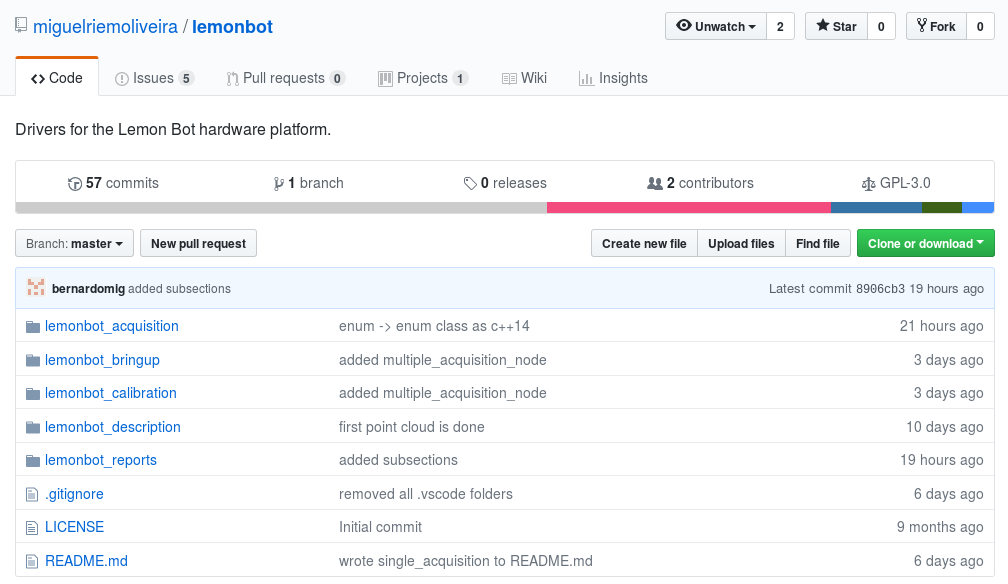
\includegraphics[width=\textwidth]{img/repo.png}						
	\end{figure}
															    
\end{frame}

\begin{frame}{Packages}
			
	\begin{itemize}
		\item lemonbot\_acquisition	      
			
			\only<1>{
		      	Contem estrutura de aquisição de nuvem de pontos e imagens.
		      }
		\item lemonbot\_bringup	      
			
			\only<2> {
		      	Faz o bringup do sistema, ou seja, inicia todas as drivers e nós de controlo do sistema.
		      }
		\item lemonbot\_calibration
			
			\only<3> {
		      	Contem a informação de calibrações intrínsecas e extrínsecas do sensor e da câmara, assim como o software para a obter.
		      }	      
		\item lemonbot\_description
			
			\only<4> {
		      	Contem a informação geométrica do robot, ou seja, os \textit{urdf}/\textit{xacro} 
		      }	      
	\end{itemize}
															
\end{frame}

\begin{frame}[fragile]{Plug \& Play}
							
	Start the system:
							
\begin{lstlisting}
roslaunch lemonbot_bringup all.launch
\end{lstlisting}
						
	Single Acquisition:
						
\begin{lstlisting}
roslaunch lemonbot_acquisition single_acquisition
    type:=hybrid
    min:=-90 max:=+90 vel:=3.0
    nsteps:=20
\end{lstlisting}
							  
							        
\end{frame}

{
\usebackgroundtemplate{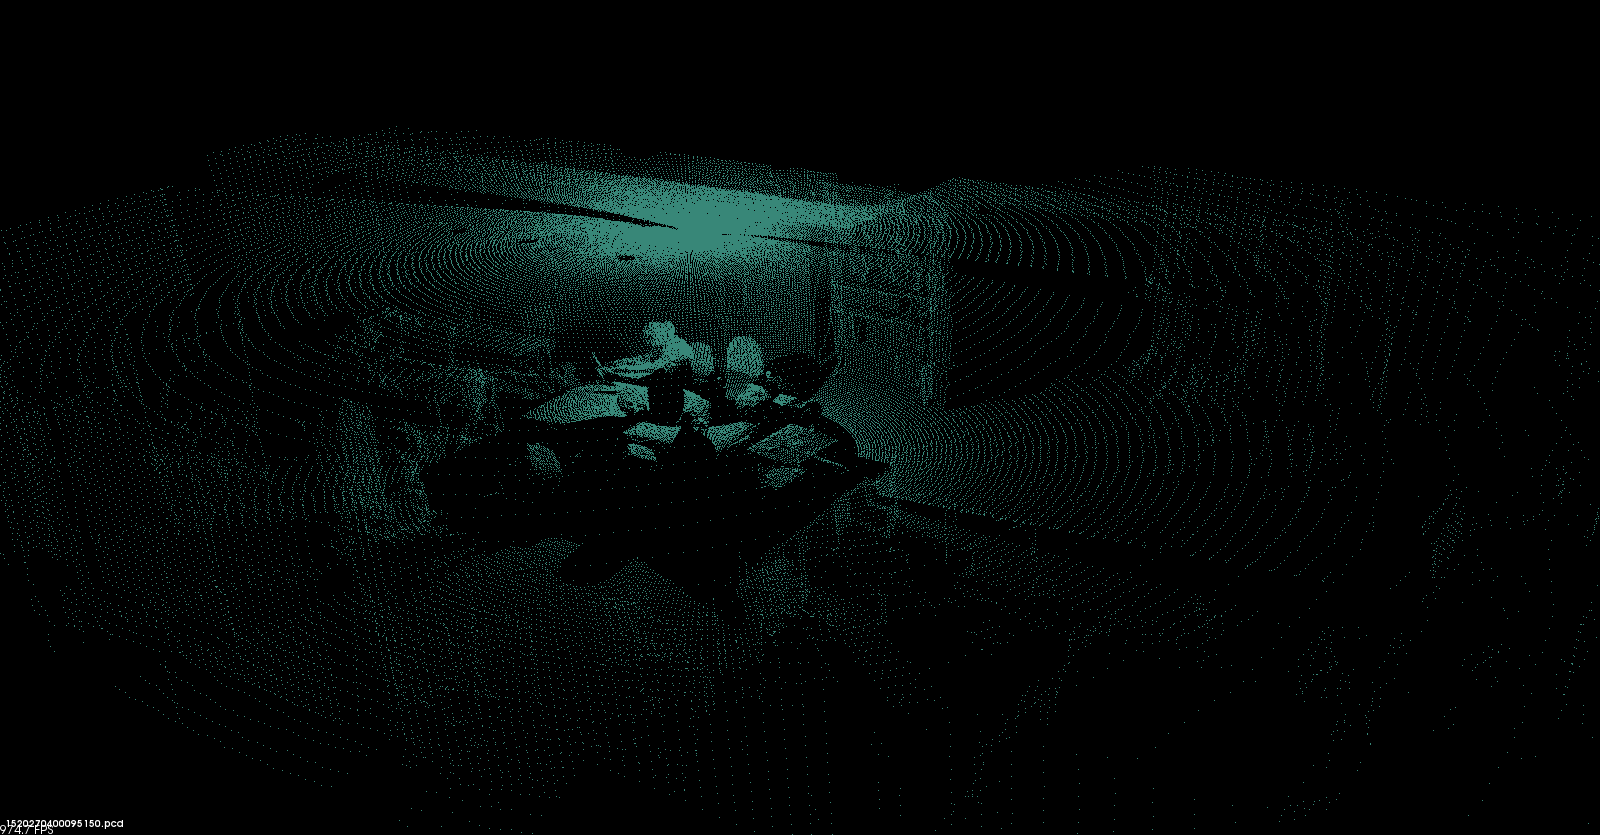
\includegraphics[height=\paperheight]{img/first-scan.png}}
\begin{frame}{Primeira Aquisição}

\end{frame}
}